\chapter{{\color{done}Изменение геострофического ветра с высотой, термический ветер}}

В целом для атмосферы характерен неравномерный нагрев с тепло в области экватора и холодом в области полюсов. Вследствие этого возникают широтные различия в поле массы. Можно ожидать, что эти различия оказывают влияние на движения в атмосфере. Так и есть. Одним из проявлений горизонтальных различий температуры является изменение геострофического ветра с высотой. В качестве элементарного приближения рассмотрим как будет происходить изменение с высотой в зависимости от температуры. Для этого запишем систему уравнений движения, применив гидростатический и геострофический балансы
\begin{align}    
    0 &= \frac{1}{\rho}\pd{p}{z}+g  \label{eq:A_TW1}  \\
    0 &= -\frac{1}{\rho}\pd{p}{x}+fv_g  \label{eq:A_TW2}  \\ 
    0 &= -\frac{1}{\rho}\pd{p}{y}-fu_g  \label{eq:A_TW3}.
\end{align}
Продифференцируем по высоте $\partial z$ уравнения движения. Запишем это на примере уравнения по $x$ (\ref{eq:A_TW3}):
\begin{equation*}
    \pd{}{z} \bigg| \:\:\: 0 = -\frac{1}{\rho}\pd{p}{x}+fv_g .
\end{equation*}
С использованием уравнения (\ref{eq:A_TW1}) и (\ref{eq:A_TW2}) получим
\begin{multline}
   0 = -\frac{1}{\rho}\pd{\rho}{z}\pd{p}{x}-
    \frac{1}{\rho} \pd{}{z} \rb{ \pd{p}{x} } + 
    f\pd{v_g}{z} = \\
  = fv_g\frac{1}{\rho}\pd{\rho}{z}-
    \frac{1}{\rho} \pd{(-\rho g)}{x} + 
    f\pd{v_g}{z} = \\
  = fv_g\frac{1}{\rho}\pd{\rho}{z}  + 
          g\frac{1}{\rho}\pd{\rho}{x} + 
          f\pd{v_g}{z}. \label{eq:A_TW4}
\end{multline}
Логарифмируем выражение уравнение состояния, держа в уме, что $\frac{1}{\rho}\pd{p}{z}=\pd{\ln{\rho}}{z}$
\begin{equation*}
    \ln{p} = \ln{\rho} + \ln{R} + \ln{T}
\end{equation*}
и дифференцируем по $z$ 
\begin{equation}
    \frac{1}{p}\pd{p}{z} = \frac{1}{\rho}\pd{\rho}{z} + \frac{1}{T}\pd{T}{z}. \label{eq:A_TW5}
\end{equation}
и по $x$
\begin{equation}
    \frac{1}{p}\pd{p}{x} = \frac{1}{\rho}\pd{\rho}{x} + \frac{1}{T}\pd{T}{x}. \label{eq:A_TW5}
\end{equation}


В подставляем в (\ref{eq:A_TW4}) выражение из (\ref{eq:A_TW5}), получим
\begin{equation}
    0 = fv_g\rb{ \frac{1}{p}\pd{p}{z} - \frac{1}{T}\pd{T}{z} } + 
    g\rb{ \frac{1}{p}\pd{p}{x} - \frac{1}{T}\pd{T}{x} } + f\pd{v_g}{z}.
\end{equation}
 Заменим $\pd{p}{z}$ гидростатическим выражением из (\ref{eq:A_TW1}), а  $\pd{p}{x}$ -- геострофическим балансом (\ref{eq:A_TW2})-(\ref{eq:A_TW3})
 \begin{multline*}
    0 = fv_g\rb{ -g - \frac{1}{T}\pd{T}{z} } + 
    g\rb{ fv_g - \frac{1}{T}\pd{T}{x} } + f\pd{v_g}{z} = \\
    = \cancel{-f v_g g} - \frac{fv_g}{T}\pd{T}{z} + \cancel{f v_g g} - \frac{g}{T}\pd{T}{x} + f\pd{v_g}{z} = - \ub{ \frac{fv_g}{T}\pd{T}{z} }_{A} - \ub{ \frac{g}{T}\pd{T}{x} }_{B} + f\pd{v_g}{z}.
\end{multline*}
Вспоминая масштабный анализ из раздела \ref{ch4.1}), рассмотрим величины отношения слагаемых $A$ и $B$
\begin{align*}
    \frac{A}{B} \sim  \frac{ \Delta T_v\cdot f\cdot U\cdot T\cdot L }{T\cdot H\cdot  g\cdot \Delta T_h} \approx \frac{6 \cdot 10^{-3} \cdot H \cdot 10^{-4} \cdot 10 \cdot 10^{3} }{ H \cdot 10 \cdot 10 } = 6 \cdot 10^{-5}.
\end{align*}
Поскольку $\Delta T_v \approx 6 \qb{^{\circ}/\textrm{км}} = 6 \cdot 10^{-3} \:\: \qb{^{\circ}/\textrm{м}}$, а $\Delta T_h \approx 10\qb{^{\circ}/L }$ (см. рис. \ref{fig:A_TW1}). Значит слагаемое $A$ на 5 порядков меньше, следовательно его можно отбросить. 

Вывод для остальных компонент производится аналогично, поэтому запишем сразу итоговое уравнение для термического ветра
\begin{align}
    \pd{v_g}{z} &= \frac{g}{Tf}\pd{T}{x} \label{eq:A_TWV} \\
    \pd{u_g}{z} &=-\frac{g}{Tf}\pd{T}{y} \label{eq:A_TWU}
\end{align}
    \begin{figure}[h]
    \centering
    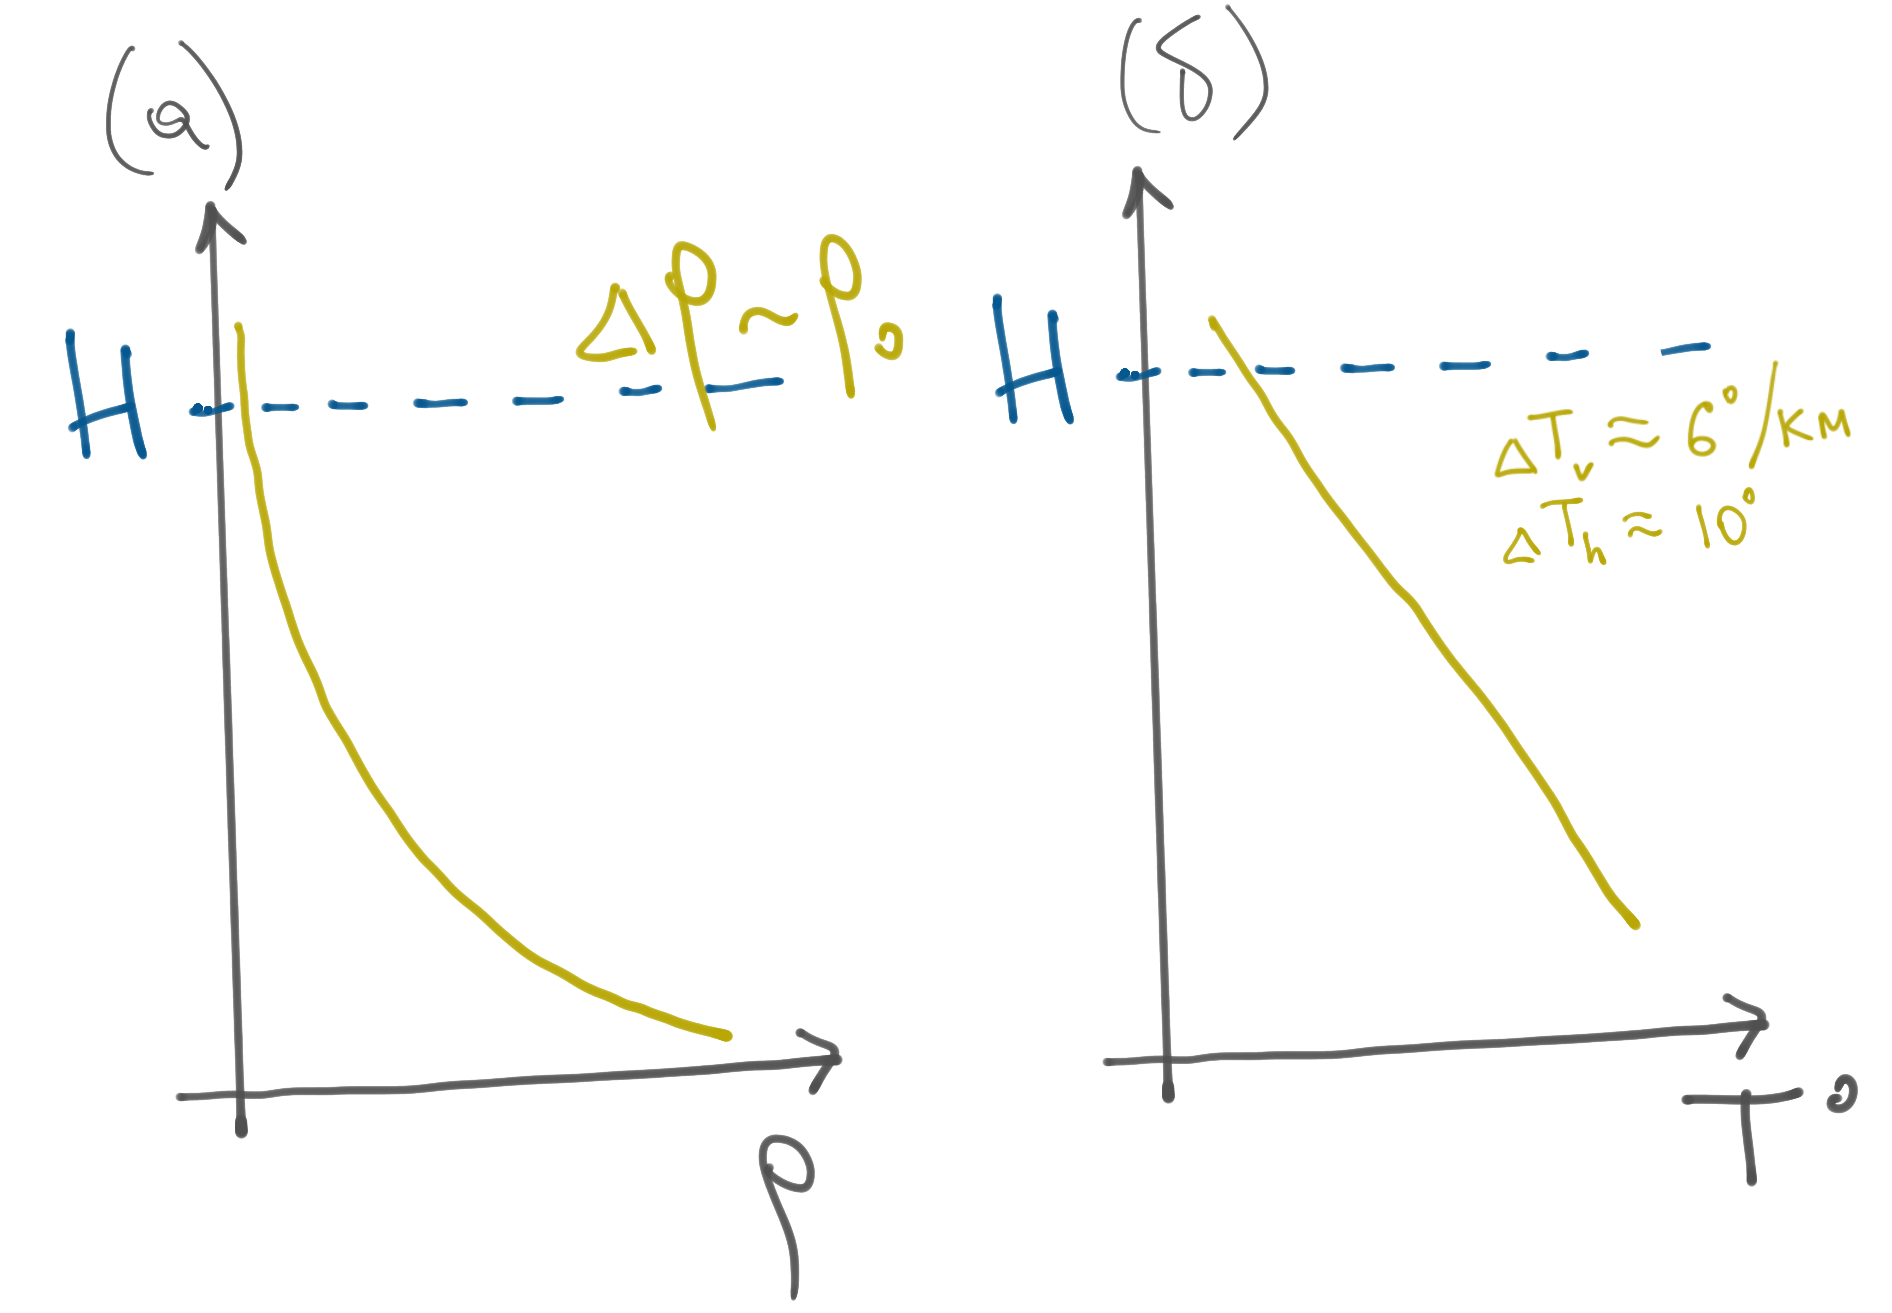
\includegraphics[width=0.3\linewidth]{pics/A_TW1.png}
    \caption{\label{fig:A_TW1}
    {\color{red} Распределение плотности (а) и температуры (б) в стандартной атмосфере. \textbf{ОПИСАТЬ!!! }}
    }
    \end{figure}    

Физический смысл термического ветра есть изменение ветра с высотой по действием горизонтальной неоднородности распределения температуры. Покажем это проинтегрировав (\ref{eq:A_TWV}) и (\ref{eq:A_TWU}) по вертикали (для компоненты $u_g$) и произведем нормирование на $\Delta z$
\begin{equation*}
    \ub{\frac{1}{z_2-z_1}}_{\Delta z} \int_{z_1}^{z_2} \:\:\:  \bigg| \:\:\: \pd{u_g}{z} =-\frac{g}{Tf}\pd{T}{y} \:\:\: \bigg| \:\:\: dz
\end{equation*}
Получим
\begin{equation*}
    \frac{1}{\Delta z} \qb{u_g(z_2) - u_g(z_1) } \simeq -\frac{g}{\overline{T}f}\pd{\overline{T}}{y},
\end{equation*}
где $\overline{T}$ -- это средняя температура в слое $\rb{ \overline{T} = \frac{1}{\Delta z} \int_{z_1}^{z_2} T dz  } $. Домножим получившееся уравнение на $\Delta z$ 
\begin{equation}
    \Delta u_g = -\frac{g}{\overline{T}f } \pd{}{y} \qb{ \int_{z_1}^{z_2} T dz }.
\end{equation}
Эту формулу уже удобно интерпретировать. Допустим на высоте $z_1$ изобара проходит параллельно высоте (рис. $\ref{fig:A_TW2}$). Возьмем вертикальный срез атмосферы от юга до севера (ось $y$ направлена на север). Тогда, исходя из (\ref{eq:A_TW3}), скорость геострофического ветра на высоте $z_1$ будет равняться нулю. Поскольку на юге теплее, чем на севере, то изобара на высоте $z_2$ будет наклонена к полюсу, значит широтный температурный градиент будет меньше нуля $\rb{ \pd{T}{y}<0 }$, следовательно $\Delta u_g >0$. То есть, в условиях существования горизонтального градиента давления, скорость геострофического ветра получает добавок (в рассмотренном идеализированном случае положительный). 
    \begin{figure}[h]
    \centering
    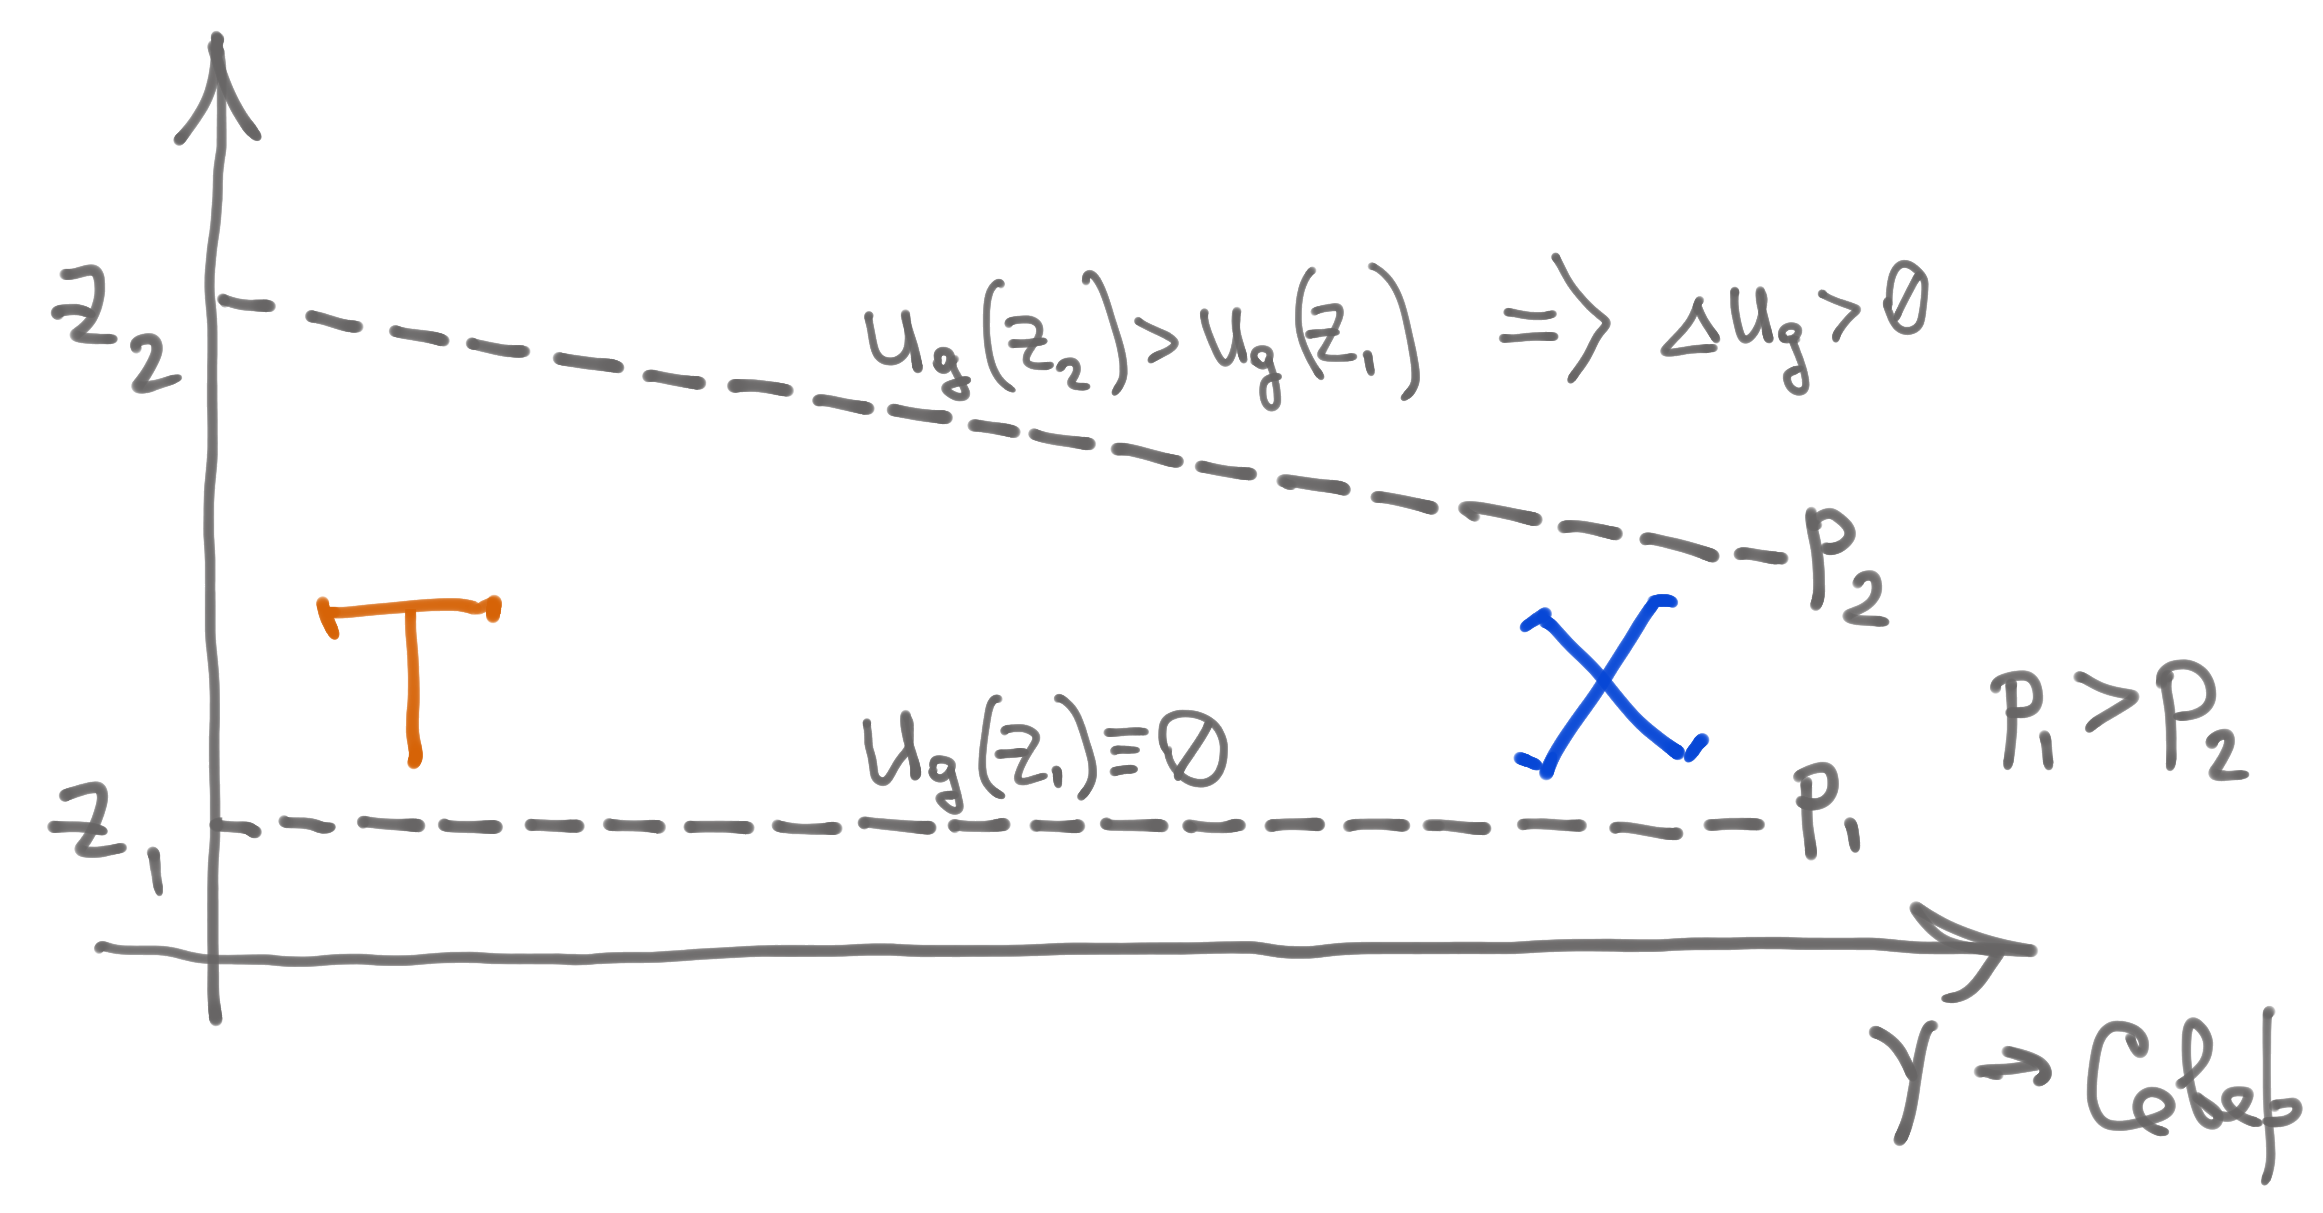
\includegraphics[width=0.7\linewidth]{pics/A_TW2.png}
    \caption{\label{fig:A_TW2}
    {\color{red} Схема действия термического ветра}
    }
    \end{figure}    
Если оперировать общими закономерностями, что в высоких широтах всегда холоднее, чем на экваторе. Значит изотермы в каждом из полушарий направленны как на рисунке $\ref{fig:A_TW2}$. Таким образом, термический ветер {\color{red} создает} западный перенос. 

Так как в целом в тропосфере холод имеет место у полюсов, можно ожидать, что с высотой будет увеличиваться западная составляющая ветра. Если бы характерный для тропосферы температурный градиент наблюдался до верхней границы атмосферы, то скорость западных потоков увеличивалась. Однако градиент температуры меняет знак в стратосфере, поэтому сдвиг геострофического ветра меняет знак и западные потоки достигают максимума на тропопаузе. Далее, градиенты температуры в тропосфере концентрируются в бароклинных фронтальных  зонах, поэтому и термический ветер  наиболее хорошо выражен в этих бароклинных зонах, где достигается максимум западного переноса и образуются струйные течения вблизи тропопаузы. Эффект термического ветра приводи также к тому, что ветер на высотах является более гладким, чем у поверхности Земли. В баротропной атмосфере возмущения, возникшие вблизи земной поверхности, распространились бы по всей толще атмосферы. 

С термическим ветром связан характер геострофической термической адвекции. Если мы находимся в фиксированной точке, то локальные изменения температуры за счет адвекции будут иметь вид 
\begin{equation}
    \label{eq:ch12_js1}
    \pd{T}{t} = -u\pd{T}{x}-v\pd{T}{y}.
\end{equation}
Если заменить скорости в правой части геострофическими скоростями и представить последние в членах градиентов давления с использованием геострофического ветра, то получим

\begin{equation}
    \label{eq:ch12_js2}
    \pd{T}{t} = -\frac{1}{f\rho} \rb{ \pd{p}{x}\pd{T}{y} - \pd{p}{y}\pd{T}{x} }.
\end{equation}
Выражение в скобках представляет собой векторные произведения горизонтальных векторов $\pd{p}{n}$ и $\pd{T}{m}$, поэтому

\begin{equation}
    \label{eq:ch12_js3}
    \pd{T}{t} = -\frac{1}{f\rho}\pd{p}{n}\pd{T}{m} \sin{\alpha},
\end{equation}
где $\alpha$ -- угол между горизонтальными градиентами давления и температуры (см. рис. \ref{fig:ch12.1})

    \begin{figure}[h]
    \centering
    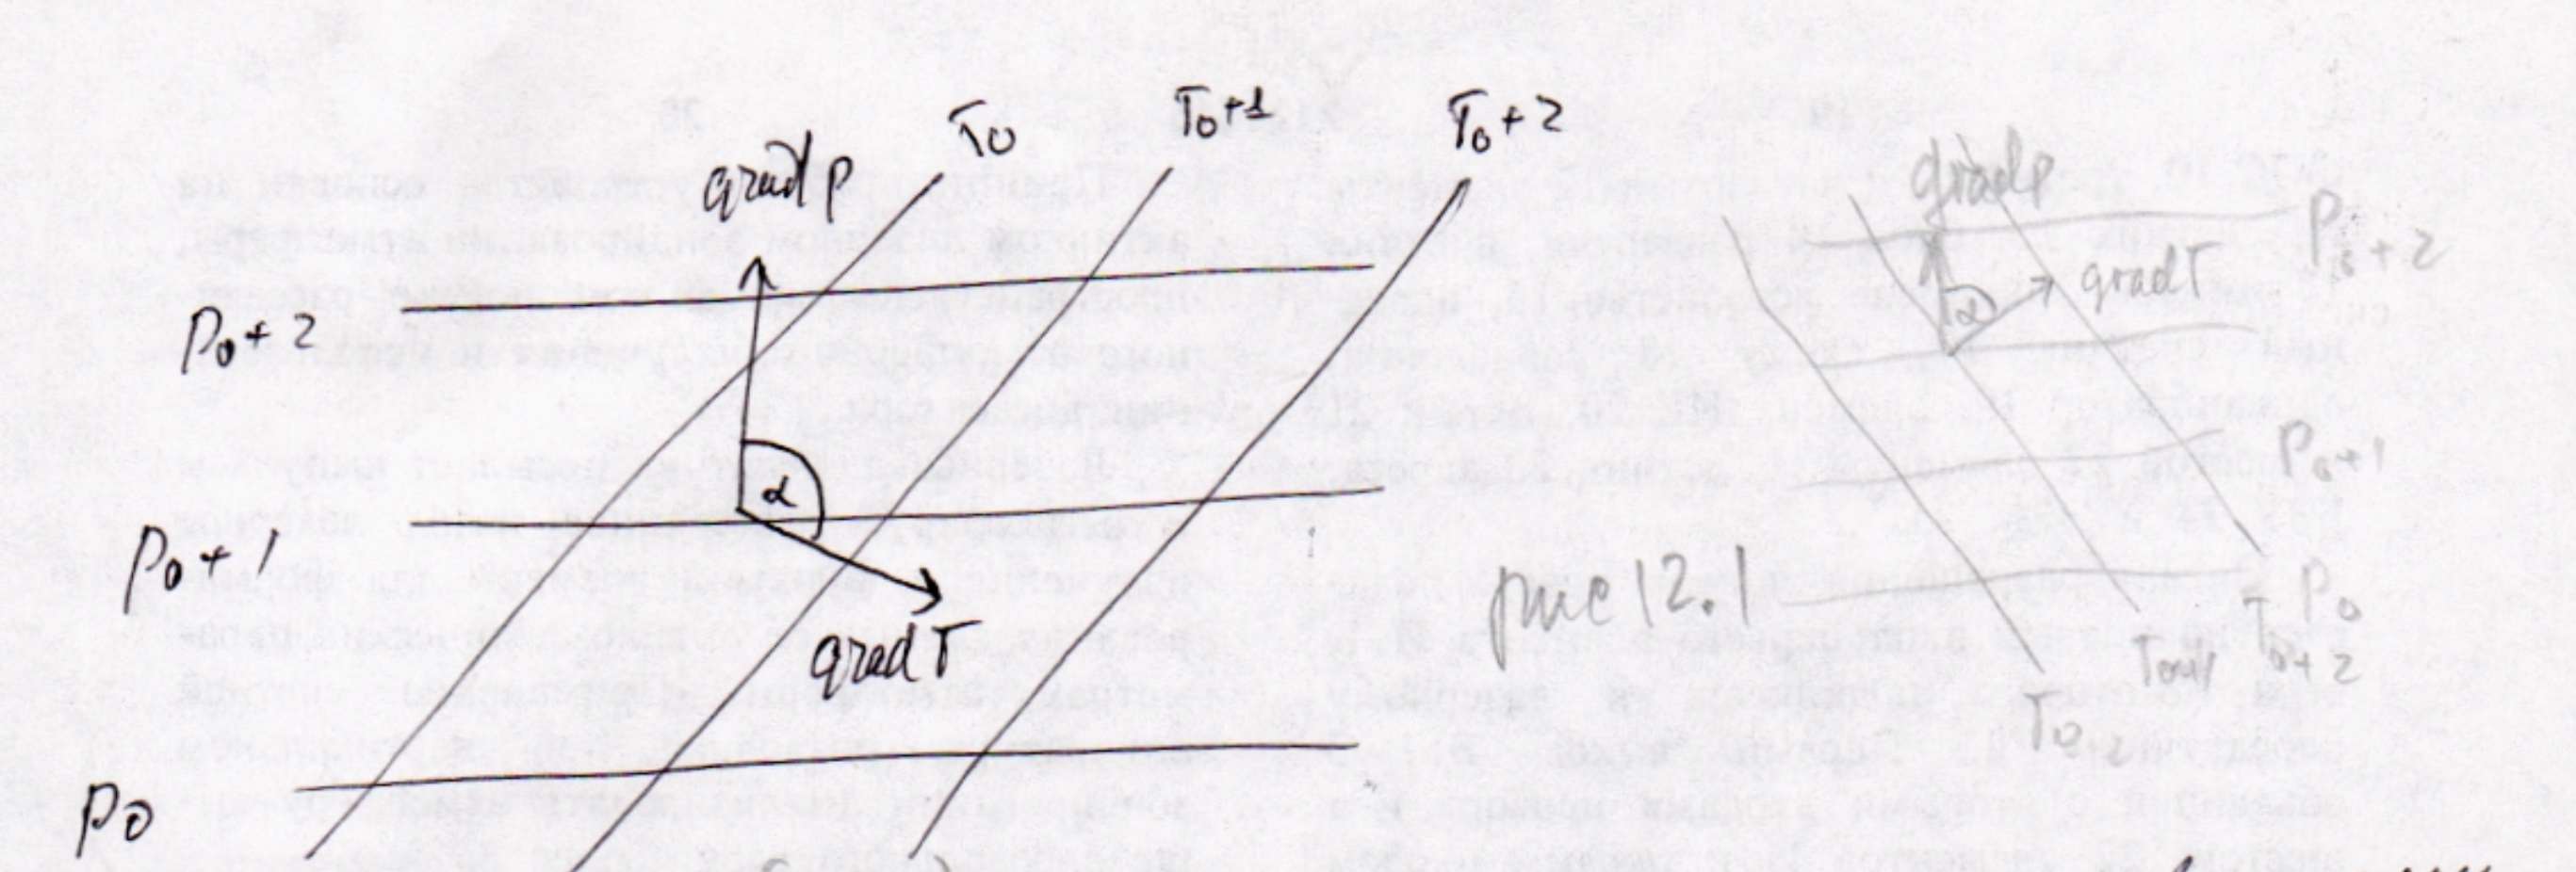
\includegraphics[width=0.7\linewidth]{pics/ch12.1.png}
    \caption{\label{fig:ch12.1}
    {\color{red} \textbf{ОПИСАТЬ!}}
    }
    \end{figure}    

Из формулы \ref{eq:ch12_js3} вытекает (применительно к северному полушарию, где $f>0$), что левому повороту ветра с высотой ($\alpha>0$) соответствует отрицательная геострофическая адвекция температуры (адвекция холода), а правому повороту ветра ($\alpha<0$) --  положительная геострофическая адвекция (адвекция тепла). Здесь предполагается, что $\alpha$ изменяется от $0$ до $\pm\frac{\pi}{2}$.

Левый поворот означает поворот против часовой стрелки (от вектора градиента температуры к вектору градиента давления), а правый поворот -- по часовой стрелке (см. рис. \ref{fig:ch12.2}).

    \begin{figure}[h]
    \centering
    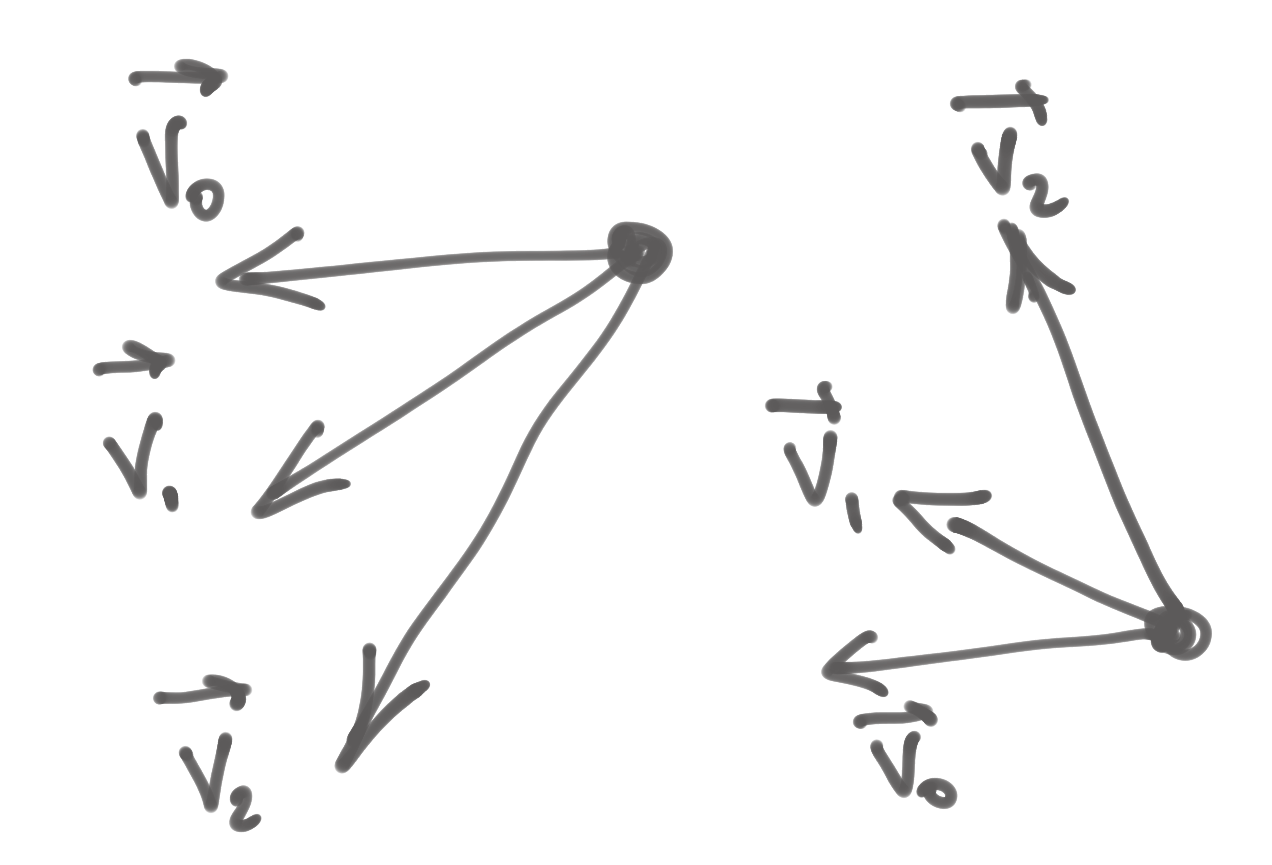
\includegraphics[width=0.5\linewidth]{pics/ch12.2.png}
    \caption{\label{fig:ch12.2}
    {\color{red} \textbf{ОПИСАТЬ! Сказать про нумерацию векторов по высоте слоев.}}
    }
    \end{figure}    

    \begin{figure}
    \begin{minipage}[b]{.52\textwidth} % left
        \centering
        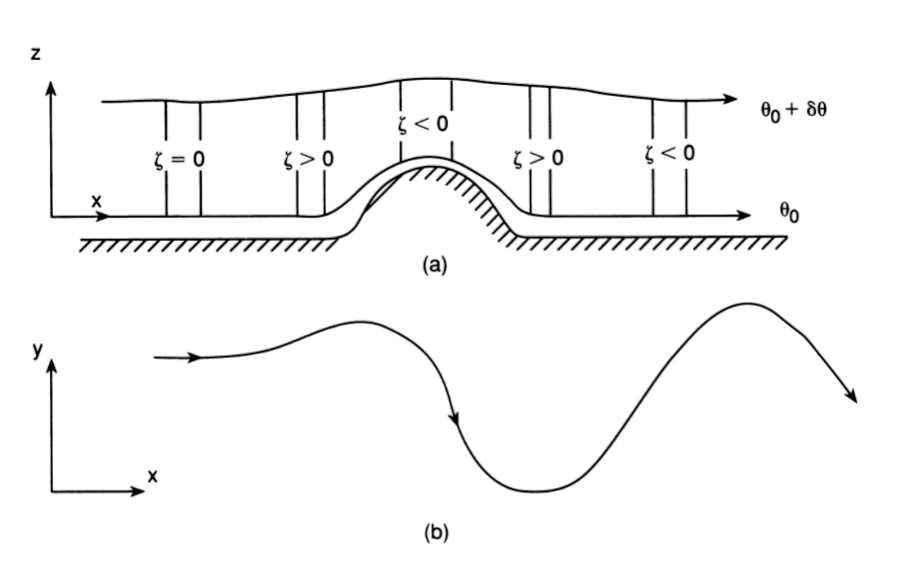
\includegraphics[width=1\linewidth]{pics/ch12.31.png}
        \end{minipage}%
    \begin{minipage}[b]{.48\textwidth} % right
      \centering
      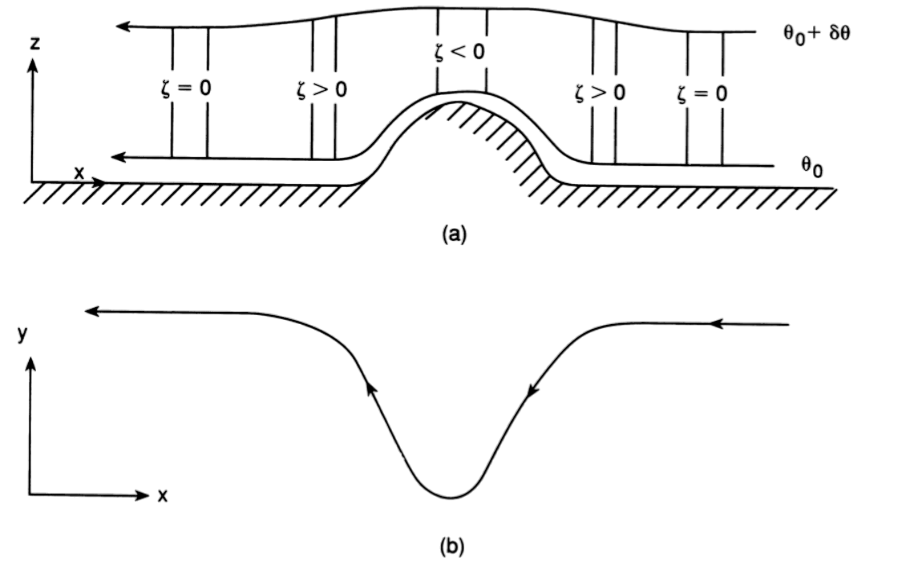
\includegraphics[width=1\linewidth]{pics/ch12.32.png}
    \end{minipage}
    \caption{\label{fig:ch12.3} {\color{red}Схема обтекания препятствия и сохранение потенциальной завихренности}}
    \end{figure}



Следует отметить что, определение <<термический ветер>> -- это именно сдвиг ветра с высотой, а не ветер в обычном понимании этого слова. Тем не менее это вектор с размерностью скорости. Также, система уравнений гидростатики и геострофическое приближение дает уравнение термического ветра. Следовательно, пределы применимости термического ветра -- для синоптического и более масштабов.
